\chapter{Header und Footer}

In Latex ist es möglich die Seiteneinstellung anzupassen. Unter anderem können die Kopfzeile und Fußzeile angepasst werden. Die Anpassungsmöglichkeiten beziehen sich auf die Breite und Höhe sowie Inhalt der Zeilen. Umgesetzt wird dies in der Praxis mit den Paketen \emph{fancyhdr} und \emph{titleps}. 

\begin{description}
	\item[fancyhdr:] Das Paket bietet umfangreiche Möglichkeiten, sowohl für die Erstellung von Kopf- und Fußzeilen als auch für die Steuerung ihrer Verwendung (z.B. in Zeiten, in denen LATEX automatisch den verwendeten Überschriften-Stil ändert).\\
	\url{https://ctan.org/pkg/fancyhdr}
	\item[titleps:] Das Paket bietet Seitenstile mit einem einfachen einstufigen Mechanismus, einschließlich Bestnoten, Zugriff auf Top-, First- und Botmarks in einem einzigen Header/Footer, Header/Footer für bestimmte Floats, mehrere Sätze von Marken (mit e-TEX) und mehr.
	Das Paket ist Teil der titleec-Distribution.\\
	\url{https://ctan.org/pkg/titleps}
\end{description}

Im ersten Beispiel wird die generelle Nutzung gezeigt von \emph{fancyhdr}. Das Ergebnis des LaTeX Quellcodes wird mit dem package \emph{pdfpages} eingebunden. Im zweiten Beispiel wird gezeigt wie in der Fußzeile die aktuelle Seitenzahl zur Gesamtanzahl der Seiten mit Hilfe des Paketes \emph{lastpage} angezeigt werden kann.
\newpage
\begin{lstlisting}[style=LaTeX]
\documentclass[12pt]{article}
\usepackage{titleps} % für die Seitenstile
\usepackage{fancyhdr} % für die Kopfzeile und Fußzeile
\usepackage{graphicx} % für das example-iamge-a
\usepackage{lipsum} % für dummy text

\pagestyle{myheadings}
\pagestyle{fancy}
\fancyhf{}

\setlength{\headheight}{30pt} % Höhe der Kopfzeile

\renewcommand{\headrulewidth}{4pt} % Dicke der Kopzeile
\renewcommand{\footrulewidth}{2pt} % Dicke der Fußzeile

\fancyhead[L]{\includegraphics[width=1cm]{example-image-a}}
\fancyhead[C]{} % Option C bedeutet Center wie (L)eft
\fancyhead[R]{\rightmark}
\fancyfoot[L]{ABC}
\fancyfoot[C]{\textcopyright xyz}
\fancyfoot[R]{\thepage}


\begin{document}

\section{First section}
\subsection{One}
\lipsum[1-3]
\subsection{Two}
\lipsum[4-6]

\end{document}
\end{lstlisting}

% Package pdfpages https://www.namsu.de/Extra/pakete/Pdfpages.html
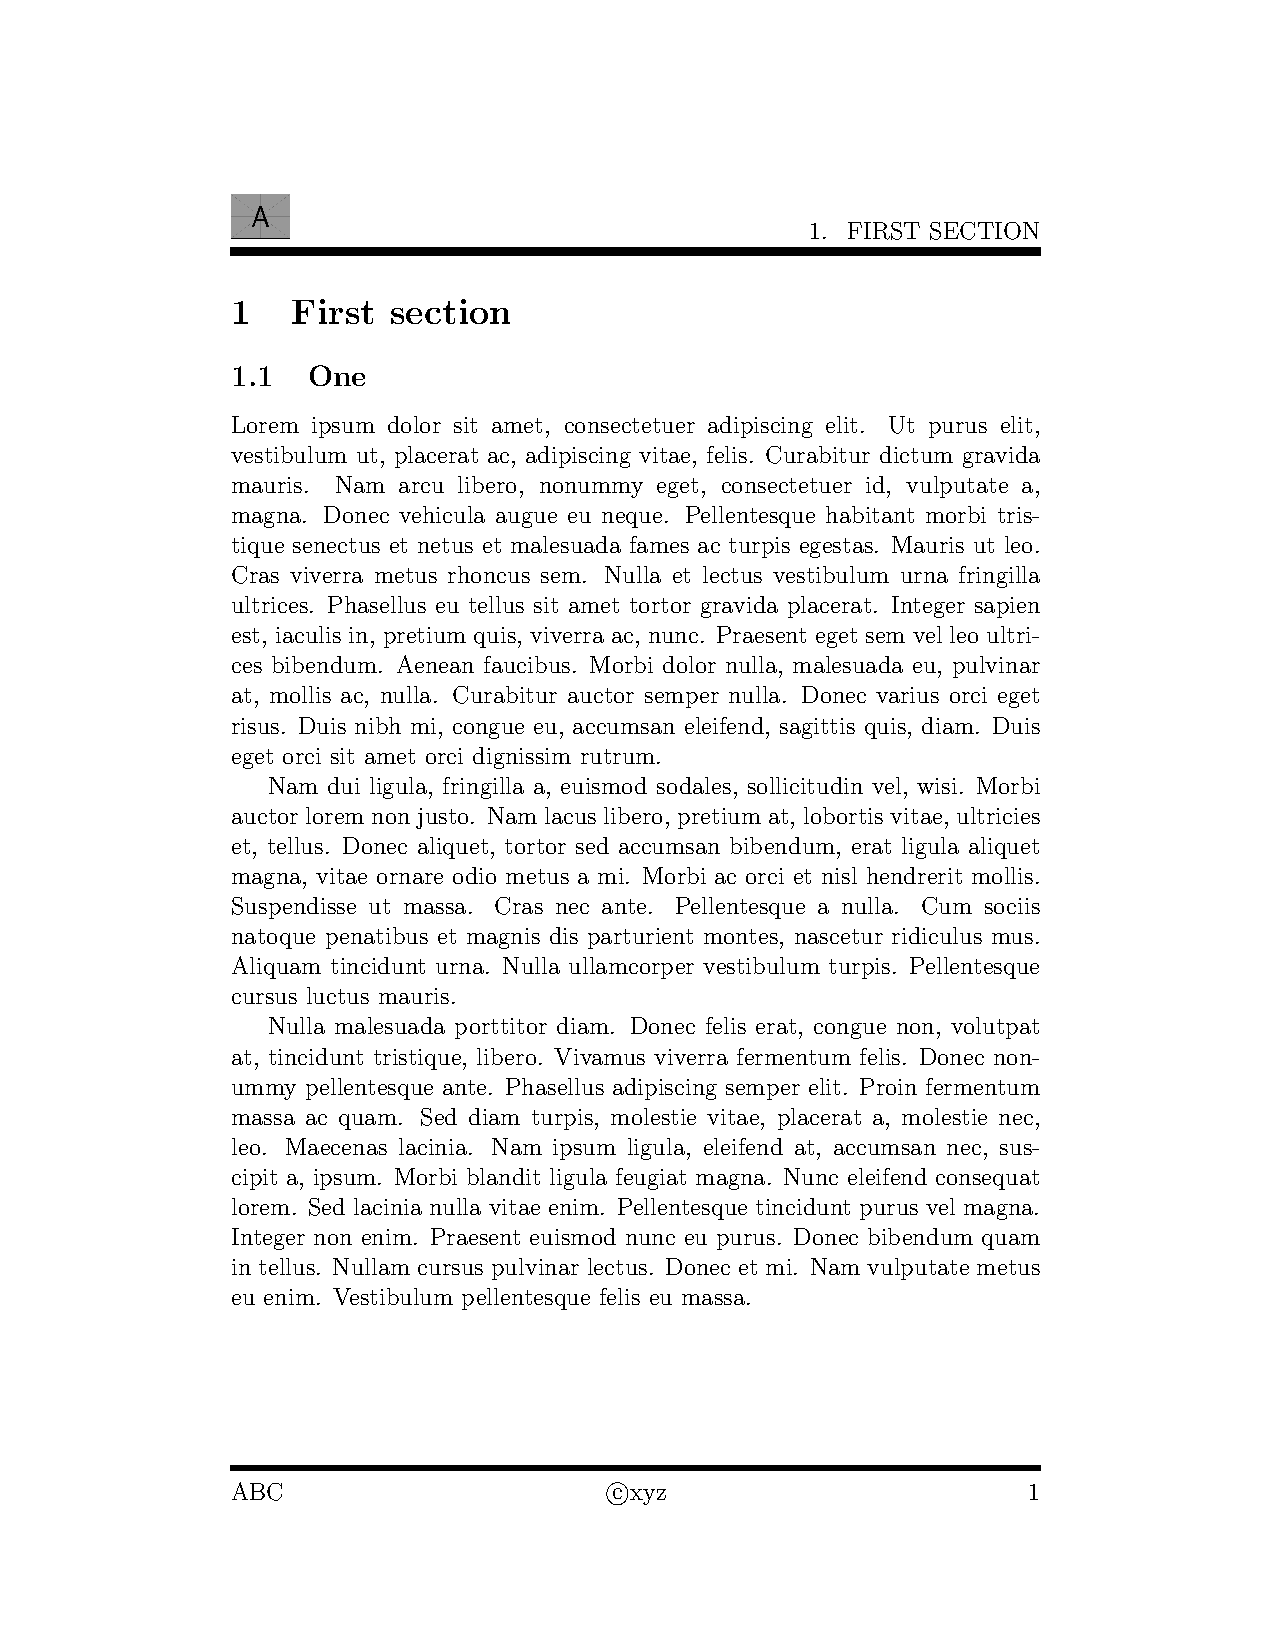
\includepdf[pages=-]{examples/header-footer} 

\begin{lstlisting}[style=LaTeX]
\documentclass[12pt]{article}
\usepackage{lastpage}
\usepackage{fancyhdr}
\usepackage{graphicx}
\usepackage{lipsum} % for dummy text
\pagestyle{myheadings}
\pagestyle{fancy}
\fancyhf{}
\setlength{\headheight}{30pt}
\renewcommand{\headrulewidth}{1pt}
\renewcommand{\footrulewidth}{2pt}
\lhead{\includegraphics[width=1cm]{example-image-a}}
\rhead{}
\lfoot{ABC}
\rfoot{\thepage/\pageref{LastPage}}
\begin{document}
\subsection{One}
\lipsum[1-3]
\subsection{Two}
\lipsum[4-6]
\end{document}
\end{lstlisting}

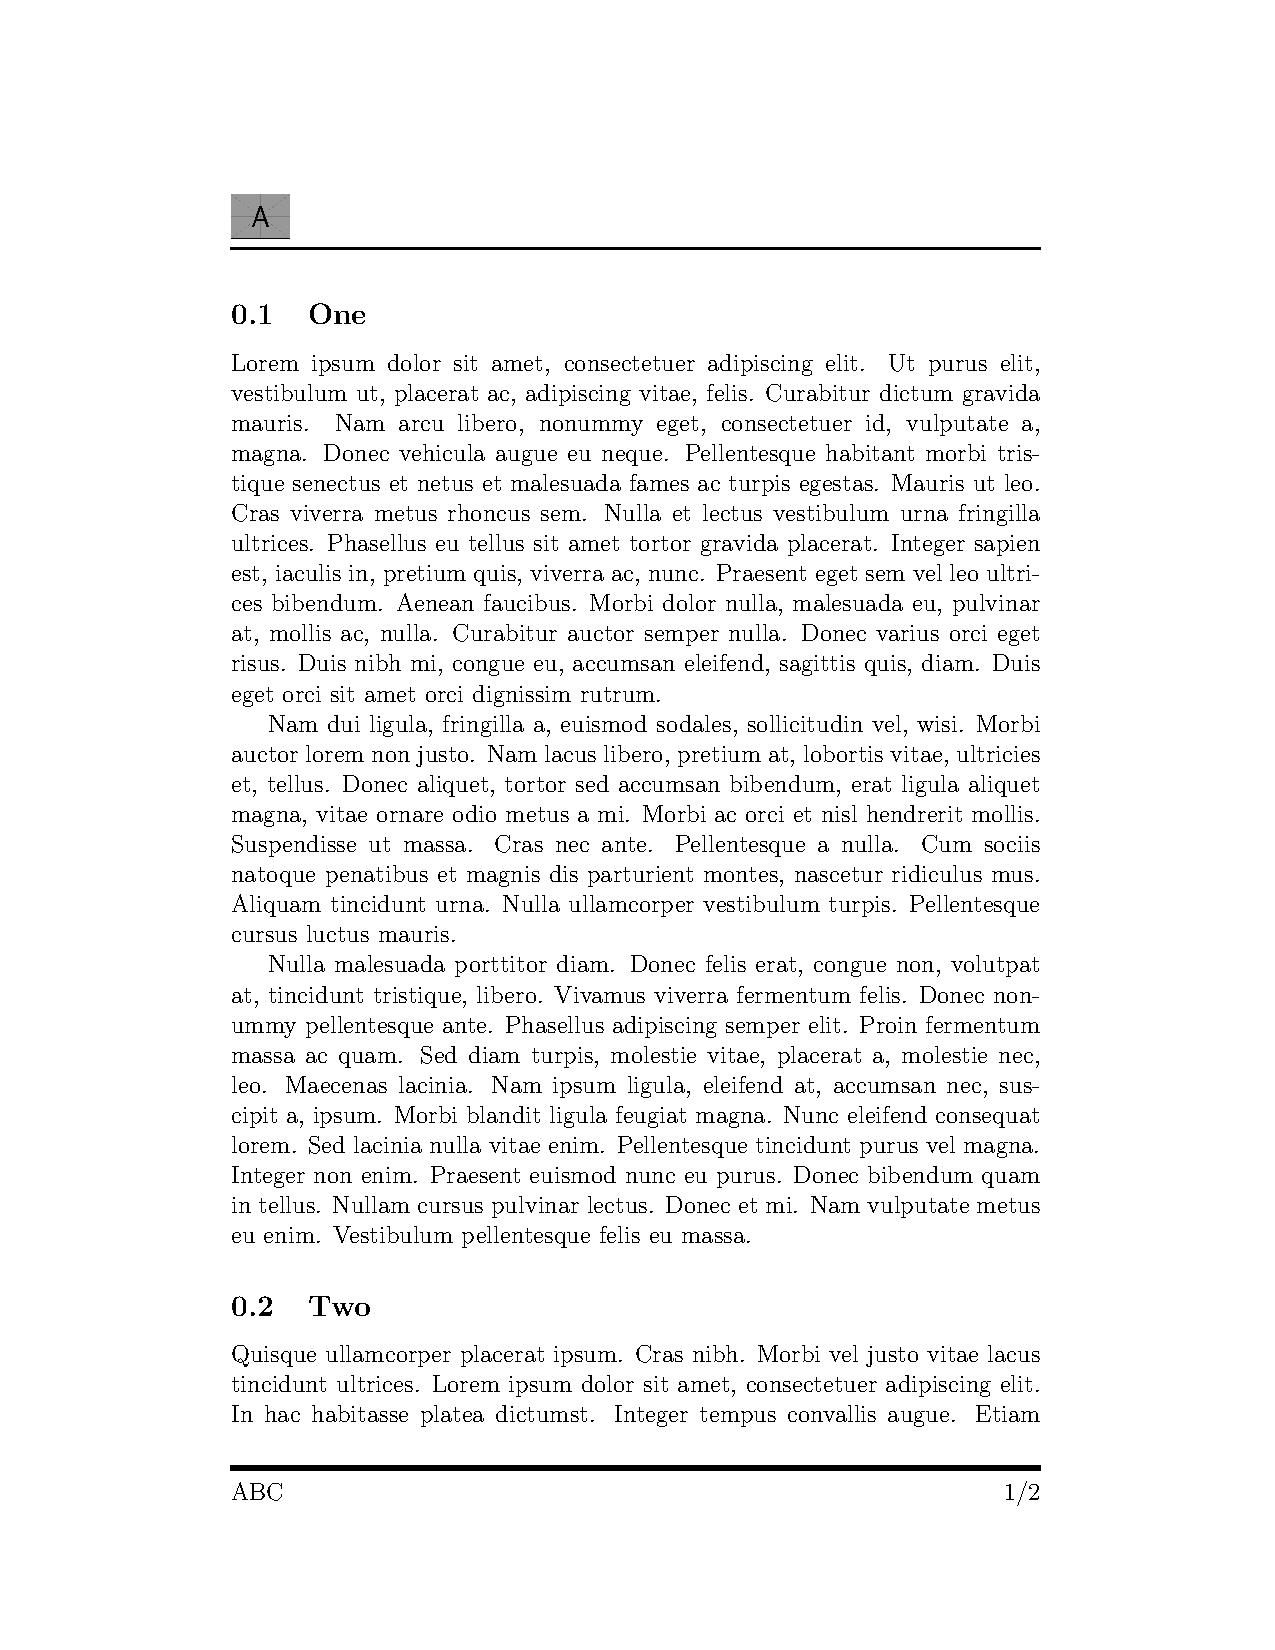
\includepdf[pages=-]{examples/header-footer-lastpage} 
